\section{Using Project-Join Trees for Weighted Model Counting}
\label{sec_jointree}

In model counting, a Boolean formula is often given in conjunctive normal form (CNF), \ie, as a set $\phi$ of clauses.
For each clause $c \in \phi$, define $\vars(c)$ to be the set of variables appearing in $c$.
Then $c$ represents a Boolean function over $\vars(c)$. Similarly, $\phi$ represents a Boolean function over $\vars(\phi) \equiv \bigcup_{c \in \phi} \vars(c)$. 

It is well-known that weighted model counting can be performed through a sequence of projections and joins on pseudo-Boolean functions \cite{DPV20,DDV19}.
Given a CNF formula $\phi$ and a literal-weight function $W$ over a set $X$ of variables, the corresponding weighted model count can be computed as follows:
\begin{equation}
\label{eq_factored_wmc}
    W(\phi) = \pars{
        % \proj_{x_1} \cdots \proj_{x_n}
        \proj_X
        \pars{\prod_{c \in \phi} c \mult \prod_{x \in X} W_x}
    }(\emptyset)
\end{equation}

% TODO: Define W_x
It was shown in \cite{DPV20} that the computational cost of Equation \ref{eq_factored_wmc} can be significantly reduced using \emph{early projection} \cite{MPPV04}. The key idea is that, when performing a product followed by a projection, it is sometimes possible to perform the projection first. Formally:
\begin{theorem}[Early Projection]
\label{thm_early_proj}
    Let $X$ and $Y$ be sets of variables.
    For all functions $f: 2^X \to \R$ and $g: 2^Y \to \R$, if $x \in X \setminus Y$, then $\proj_x (f \mult g) = \pars{\proj_x f} \mult g.$
\end{theorem}
\begin{proof}
    By Definition \ref{def_mult} and Definition \ref{def_sum}. See \textbf{Theorem 2} of \cite{DPV20} for details.
\end{proof}

Early projection is a key technique in symbolic computation in a variety of settings, including database-query optimization \cite{KV00}, symbolic model checking \cite{burch1991symbolic}, satisfiability solving \cite{pan2005symbolic}, and model counting \cite{DPV20}.

By taking advantage of the associative and commutative properties of multiplication as well as the commutative property of $\Sigma$-projection, \cite{DPV20} rearranged Equation \eqref{eq_factored_wmc} to apply early projection.
There are a variety of possible rearrangements of Equation \eqref{eq_factored_wmc} of varying computational cost.
Although \cite{DPV20} considered several heuristics for performing this rearrangement (using bucket elimination \cite{dechter99} and Bouquet's Method \cite{bouquet1999gestion}), they did not attempt to analyze rearrangements.

In this chapter, we aim to analyze the quality of the rearrangement, in isolation from the underlying implementation and data structure used for Equation \eqref{eq_factored_wmc}.
This approach has been highly successful for database-query optimization \cite{MPPV04}, where the central object of theoretical reasoning is the \emph{query plan}.
The approach has also seen similar success in Bayesian network inference \cite{darwiche1998dynamic}.

We model a rearrangement of Equation \eqref{eq_factored_wmc} as a \emph{project-join tree}:
\begin{definition}[Project-Join Tree]
\label{def_jointree}
    Let $\phi$ be a CNF formula.
    A \emph{project-join tree} of $\phi$ is a tuple $(T, r, \gamma, \pi)$ where:
    \begin{itemize}
        \item $T$ is a tree with root $r \in \V{T}$,
        \item $\gamma: \Lv{T} \to \phi$ is a bijection between the leaves of $T$ and the clauses of $\phi$, and
        \item $\pi: \V{T} \setminus \Lv{T} \to 2^{\vars(\phi)}$ is a labeling function on internal nodes.
    \end{itemize}
    Moreover, $(T, r, \gamma, \pi)$ must satisfy the following two properties:
    \begin{enumerate}[ref=\arabic*]
        \item $\{\pi(n) : n \in \V{T} \setminus \Lv{T} \}$ is a partition of $\vars(\phi)$, and \label{prop1}
        \item for each internal node $n \in \V{T} \setminus \Lv{T}$, variable $x \in \pi(n)$, and clause $c \in \phi$ \st{} $x$ appears in $c$, the leaf node $\gamma^{-1}(c)$ must be a descendant of $n$ in $T$. \label{prop2}
    \end{enumerate}
\end{definition}
If $n$ is a leaf node, then $n$ corresponds to a clause $c = \gamma(n)$ in Equation \eqref{eq_factored_wmc}.
If $n$ is an internal node, then $n$'s children $\C{T}{r}{n}$ are to be multiplied before the projections of variables in $\pi(n)$ are performed.
The two properties ensure that the resulting expression is equivalent to Equation \eqref{eq_factored_wmc} using early projection.
See Figure \ref{fig_join_tree} for a graphical example of a project-join tree.
\begin{figure}%[H]
    \centering
    \begin{tikzpicture}[grow=right] % use '~' for space; ' ' would crash
        \tikzset{level distance=80pt,sibling distance=-6pt}
        \tikzset{execute at begin node=\strut}
        \tikzset{every tree node/.style={anchor=base west}}
        \Tree [ .$n_{8}\piMap\emptyset$
            [ .$n_{7}\piMap\set{x_3, x_4}$
                [ .$n_{6}\piMap\set{x_1}$
                    [ .$n_4\gammaMap{x_1 \vee x_3 \vee \neg x_4}$ ]
                    [ .$n_3\gammaMap{\neg x_1 \vee \neg x_3}$ ]
                ]
                [ .$n_2\gammaMap{x_3 \vee x_4}$ ]
            ]
            [ .$n_{5}\piMap\set{x_2}$ [ .$n_1\gammaMap{\neg x_2}$ ] ]
        ]
    \end{tikzpicture}
\caption{
    A project-join tree $(T, n_{8}, \gamma, \pi)$ of a CNF formula $\phi$.
    Each leaf node is labeled by $\gamma$ with a clause of $\phi$.
    Each internal node is labeled by $\pi$ with a set of variables of $\phi$.
}
\label{fig_join_tree}
\end{figure}

Project-join trees have previously been studied in the context of database-query optimization \cite{MPPV04}.
Project-join trees are also closely related to contraction trees in the context of tensor networks \cite{EP14,DDV19}.
Once a rearrangement of Equation \eqref{eq_factored_wmc} has been represented by a project-join tree, we can model the computation process according to the rearrangement.
In particular, given a literal-weight function $W = \prod_{x \in X} W_x$, we define the $W$-\emph{valuation} of each node $n \in \V{T}$ as a pseudo-Boolean function associated with $n$.
The $W$-valuation of a node $n \in \V{T}$ is denoted $f^W_n$ and defined as follows:
\begin{equation}
\label{eq_valuation}
    f^W_n \equiv
    \begin{cases}
       \gamma(n) & \text{if}~n \in \Lv{T} \\
        \sum_{\pi(n)} \pars{ \prod_{o \in \C{T}{r}{n}} f^W_o \cdot \prod_{x \in \pi(n)} W_x } & \text{if}~n \notin \Lv{T}
    \end{cases}
\end{equation}

Note that the $W$-valuation of a leaf node $n \in \Lv{T}$ is a clause $c = \gamma(n) \in \phi$, interpreted in this context as an associated function $\lambda_c : 2^{\vars(c)} \to \B$ where $\lambda_c(\tau) = 1$ if and only if the truth assignment $\tau$ satisfies $c$. 

The main idea is that the $W$-valuation at each node of $T$ is a pseudo-Boolean function computed as a subexpression of Equation \eqref{eq_factored_wmc}. The $W$-valuation of the root is exactly the result of Equation \eqref{eq_factored_wmc}, \ie, the weighted model count of $\phi$ \wrt{} $W$:
\begin{theorem}
\label{thm_valuation_wmc}
    Let $\phi$ be a CNF formula, $(T, r, \gamma, \pi)$ be a project-join tree of $\phi$, and let $W$ be a literal-weight function over $\vars(\phi)$.
    Then $f^W_r(\emptyset) = W(\phi)$.
\end{theorem}

In order to prove this theorem, it is helpful to first state and prove a lemma that limits the appearance of variables in different subexpressions of Equation \ref{eq_valuation}. We also refer to this lemma in Chapter \ref{ch:procount} in the case of projected model counting.
\begin{lemma}
\label{lemma:projections_branch_disjoint}
Let $\phi$ be a CNF formula, $(T, r, \gamma, \pi)$ be a project-join tree of $\phi$, and let $W$ be a literal-weight function over $\vars(\phi)$. For each $n \in \V{T}$, denote by $S(n)$ the subtree of $T$ rooted at $n$ and further define:
\begin{align*}
    \Phi(n) &\equiv \prod_{n \in S(n) \cap \Lv{T}} \gamma(n) \\
    P(n) &\equiv \bigcup_{n \in S(n) \setminus \Lv{T}} \pi(n).
\end{align*}
For all $n \in \V{T} \setminus \Lv{T}$ and $o, o' \in \C{T}{r}{n}$, if $o \neq o'$ then $P(o) \cap \vars(\Phi(o')) = \emptyset$.
\end{lemma}
\begin{proof}
For each $x \in P(o)$, $x$ is projected out at some node below $o$ in $T$. It follows by Property 2 of Definition \ref{def_jointree} that $x$ appears in no descendent of $o'$, since $o'$ is not a descendent of $o$. Thus $P(o)$ and $\vars(\Phi(o'))$ are disjoint.
\end{proof}

We now use this lemma to prove Theorem \ref{thm_valuation_wmc}.
\begin{proof}[Proof of Theorem \ref{thm_valuation_wmc}]
Consider each $n \in \V{T}$ and define $S(n)$, $\Phi(n)$, and $P(n)$ as in Lemma \ref{lemma:projections_branch_disjoint}. The key idea is to prove for all $n \in \V{T}$ that 
$$f^W_n = \proj_{P(n)} \pars{ \Phi(n) \mult \prod_{x \in P(n)} W_x } \label{eqn:valuation:correctness}.$$
We proceed by induction on $n$ over the tree structure of $T$. In the base case, $n$ is a leaf and so $\Phi(n) = \gamma(n)$ and $P(n) = \emptyset$. So $f^W_n = \proj_{\emptyset} \pars{ \gamma(n) \mult \prod_{x \in \emptyset} W_x } = \gamma(n)$ as desired. In the inductive case, consider an internal node $n$ of $T$. By Equation \ref{eq_valuation}, $$f^W_n = \proj_{\pi(n)} \pars{\prod_{o \in \C{T}{r}{n}} f^W_o \mult \prod_{x \in \pi(n)} W_x}.$$
Plugging in the inductive hypothesis for each $f^W_o$, it follows that
$$f^W_n = \proj_{\pi(n)} \pars{\prod_{o \in \C{T}{r}{n}} \pars{\proj_{P(o)} \pars{ \Phi(o) \mult \prod_{x \in P(o)} W_{x} } } \mult \prod_{x \in \pi(n)} W_{x}}.$$
If $o, o' \in \C{T}{r}{n}$ are distinct, by Lemma \ref{lemma:projections_branch_disjoint} we know $P(o) \cap \vars(\Phi(o')) = \emptyset$. We can therefore apply Theorem \ref{thm_early_proj} to get that
$$f^W_n = \proj_{\pi(n)} \proj_{A} \pars{ \prod_{o \in \C{T}{r}{n}} \Phi(o) \mult \prod_{x \in A} W_{x} \mult \prod_{x \in \pi(n)} W_{x} }$$
where $A = \bigcup_{o \in \C{T}{r}{n}} P(o)$. Moreover, observe that $P(n) = \pi(n) \cup A$ and $\Phi(n) = \prod_{o \in \C{T}{r}{n}} \Phi(o)$. This completes the induction.

Finally, to complete the proof we observe that $P(r) = X$ and $\Phi(r) = \varphi$. It follows that $f^W_r(\emptyset) = \proj_X \pars{ \varphi \mult \prod_{x \in X} W_x } = W(\varphi)$, as desired.
\end{proof}

This gives us a two-phase algorithm for computing the weighted model count of a formula $\phi$.
First, in the \emph{planning} phase, we construct a project-join tree $(T, r, \gamma, \pi)$ of $\phi$.
We discuss algorithms for constructing project-join trees in Section \ref{sec_planning}.
Second, in the \emph{execution} phase, we compute $f^W_r$ by following Equation \eqref{eq_valuation}.
We discuss data structures for computing Equation \eqref{eq_valuation} in Section \ref{sec_execution}.

When computing a $W$-valuation, the number of variables that appear in each intermediate pseudo-Boolean function has a significant impact on the runtime.
The set of variables that appear in the $W$-valuation of a node is actually independent of $W$.
In particular, for each node $n \in \V{T}$, define $\vars(n)$ as follows:
\begin{equation}
    \vars(n) \equiv
    \begin{cases}
        \vars(\gamma(n)) & \text{if}~n \in \Lv{T} \\
        \pars{\bigcup_{o \in \C{T}{r}{n}} \vars(o)} \setminus \pi(n) & \text{if}~n \notin \Lv{T}
    \end{cases}
\end{equation}
For every literal-weight function $W$, the domain of the function $f^W_n$ is exactly $2^{\vars(n)}$.

The number of variables that appear in each intermediate pseudo-Boolean function has a significant impact on the runtime.
To characterize the difficulty of $W$-valuation, we define the \emph{size} of a node $n$, $\func{size}(n)$, to be $\size{\vars(n)}$ for leaf nodes and $\size{\vars(n) \cup \pi(n)}$ for internal nodes.
The \emph{width} of a project-join tree $(T, r, \gamma, \pi)$ is $\func{width}(T) \equiv \max_{n \in \V T} \func{size}(n)$.
We see in Section \ref{sec_experiments} how the width impacts the computation of $W$-valuations.

% Project-join trees are related to \emph{variable elimination} on factor graphs \cite{KDLD05,BDP09}, which uses tree decompositions of the primal graph of a factor graph.

% To do this, we separate the algorithm of \cite{DPV20} into two phases.
% First, in the \emph{planning} phase, we produce a rearrangement of Equation \eqref{eq_factored_wmc}.
% Second, we construct a project-join tree $(T, r, \gamma, \pi)$ of $\phi$.
% We discuss algorithms for constructing project-join trees in Section \ref{sec_planning}.
% Second, in the \emph{execution} phase, compute $f^W_r$ by following Equation \eqref{eq_valuation}.

% Although \cite{DPV20} considered various heuristics for performing this rearrangement (using bucket elimination \cite{dechter99} and Bouquet's Method \cite{bouquet1999gestion}), they did not specifically analyze the quality of the rearrangement is isolation from the underlying data structures.

% As noted in Section \ref{sec_prelim}, if $\phi: 2^X \to \{0,1\}$ is a Boolean formula and $W: 2^X \to \R$ is a pseudo-Boolean function, then $W(\phi) = \left(\sum_X (\phi \mult W) \right)(\emptyset)$.
% Moreover, \cite{DPV20} observed that, $\phi$ and $W$ can both be given in factored forms $\phi = \prod_{C_i} C_i$ (\ie, as a set of clauses) and $W = \prod_{x \in X}$ (\ie, as a literal-weight function).

% In this section, we define a project-join tree.
% We then show how a project-join tree can be used to perform weighted model counting.

% Given a CNF formula, we can construct a project-join tree, which specifies an order to apply projection and multiplication operations for model counting.

% For a project-join tree $(T, r, \gamma, \pi)$, the structure of $T$ indicates the order that multiplication should occur between the clauses at each leaf, while $\pi$ indicates the variable projections that should occur after each multiplication.
